% ============================================================
% CHAMPS -- Modeling Configuration
% ============================================================

\begin{frame}[c]{\small CHAMPS -- Modeling Configuration}
\scriptsize

\centering

\renewcommand{\arraystretch}{1.45}
\setlength{\tabcolsep}{5pt}

\begin{tabularx}{0.97\textwidth}{
    >{\centering\arraybackslash}p{0.30\textwidth}
    >{\centering\arraybackslash}X
    >{\centering\arraybackslash}X
}
\hline
\rowcolor{blue!65!black}
\color{white}\textbf{Model / Method} &
\color{white}\textbf{NACA0012} &
\color{white}\textbf{ONERA M6} \\
\hline

Turbulence Model &
Spalart--Allmaras (SA) &
Spalart--Allmaras (SA) \\
\hline

Heat-Transfer Method &
Recovery Temperature Approximation &
Recovery Temperature Approximation \\
\hline

Droplet Model &
Eulerian &
Eulerian \\
\hline

Droplet Drag Model &
Deformable Sphere &
Deformable Sphere \\
\hline

SLD Corrections &
None &
None \\
\hline

Thermodynamic Model &
Messinger &
Messinger \\
\hline

Ice Density &
Constant &
Constant \\
\hline

Surface Roughness &
Constant &
Constant \\
\hline

Geometry Evolution &
Algebraic (Single-shot) / Level Set (Multilayer) &
Algebraic (Single-shot) / Level Set (Multilayer) \\
\hline

Accretion Strategy &
Single-shot \& 5 Layers &
Single-shot \& 5 Layers \\
\hline

\end{tabularx}

\end{frame}

% ============================================================
% CHAMPS -- Capabilities and Applications
% ============================================================

\begin{frame}[c]{\small CHAMPS -- Multi-Fidelity and Multiphysics Capabilities}
\scriptsize

\begin{columns}[T,onlytextwidth]

    \begin{column}{0.49\textwidth}
        \begin{block}{\scriptsize Multi-Fidelity Aerodynamics}
            \centering
            NL-VLM $\rightarrow$ Full Potential $\rightarrow$ Euler $\rightarrow$ RANS $\rightarrow$ LES $\rightarrow$ DNS
        \end{block}
    \end{column}

    \begin{column}{0.49\textwidth}
        \begin{block}{\scriptsize Multiphysics Capabilities}
            \centering
            Fluid--Structure Interaction (FSI)
            $\quad\bullet\quad$
            Icing
            $\quad\bullet\quad$
            Contrails
        \end{block}
    \end{column}

\end{columns}

\vspace{0.15cm}

\begin{columns}[T,onlytextwidth]

    % Deterministic icing
    \begin{column}{0.19\textwidth}
        \centering
        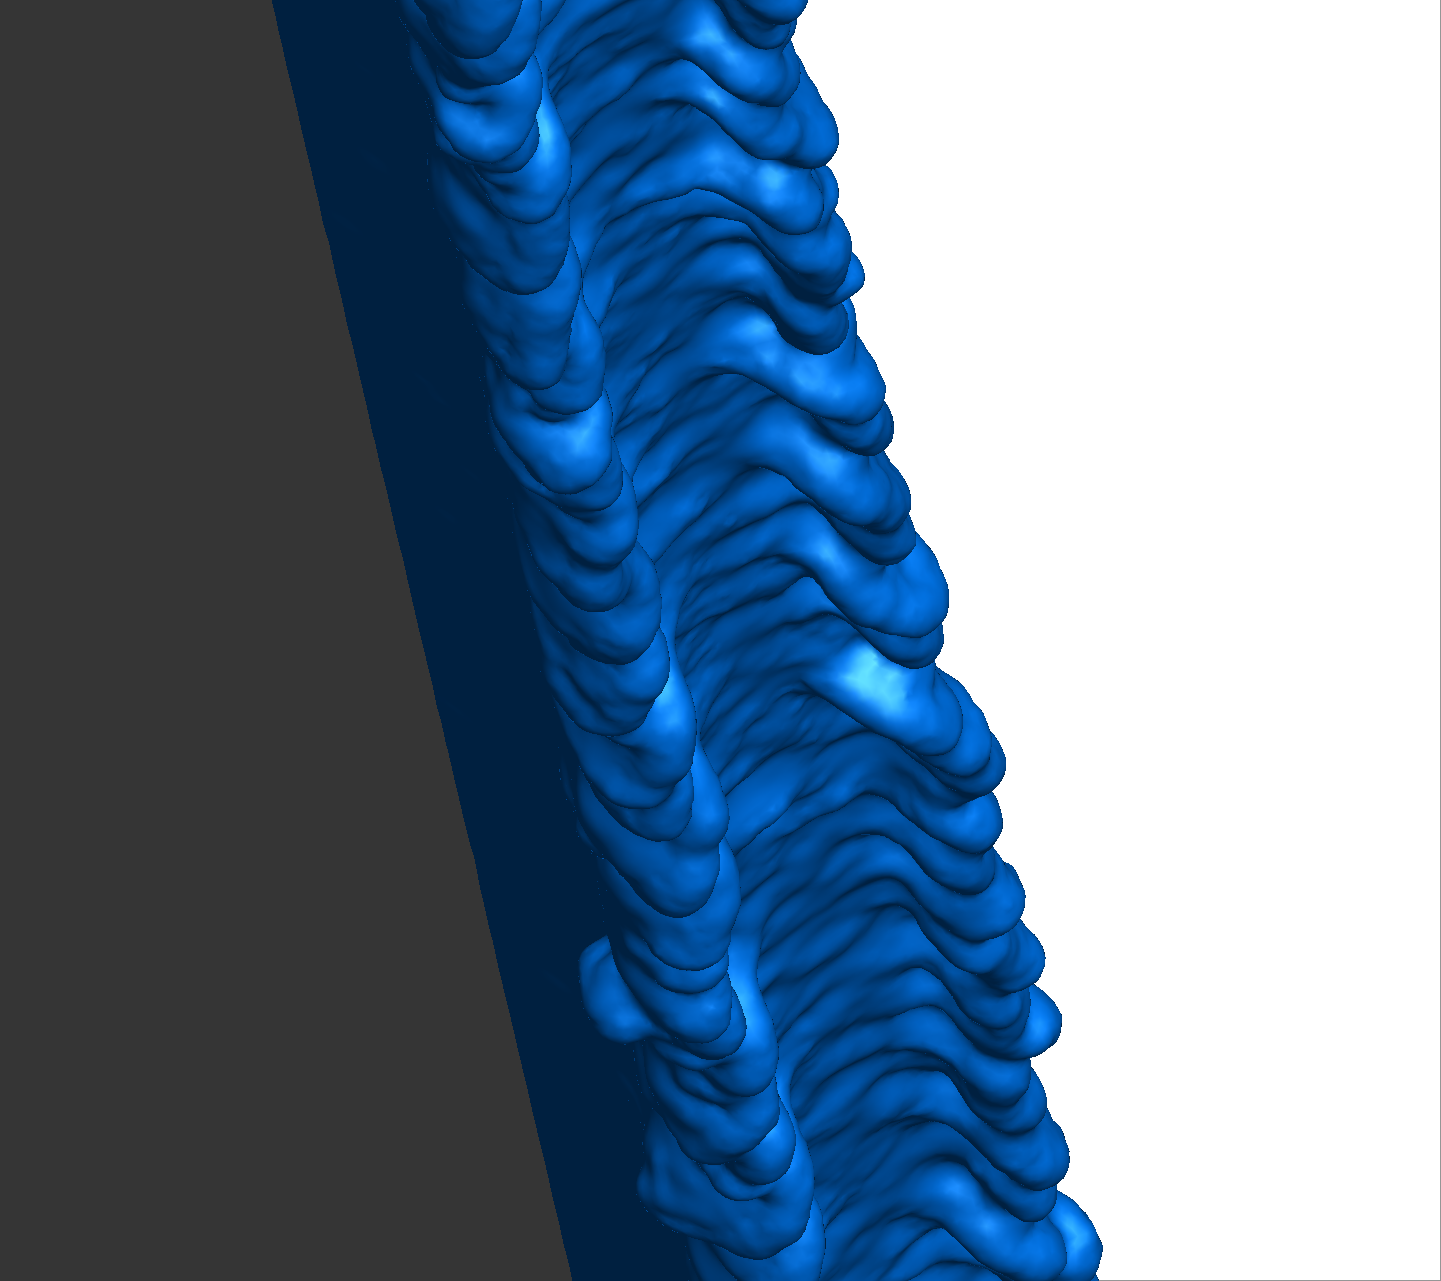
\includegraphics[width=\textwidth,height=2.65cm,keepaspectratio]
        {FIGURES/CHAMPS_APPLICATIONS/DETERMINSTIC_ICING.png}

        \vspace{0.05cm}
        \textbf{Deterministic Icing}
    \end{column}
    \hfill

    % DDES
    \begin{column}{0.19\textwidth}
        \centering
        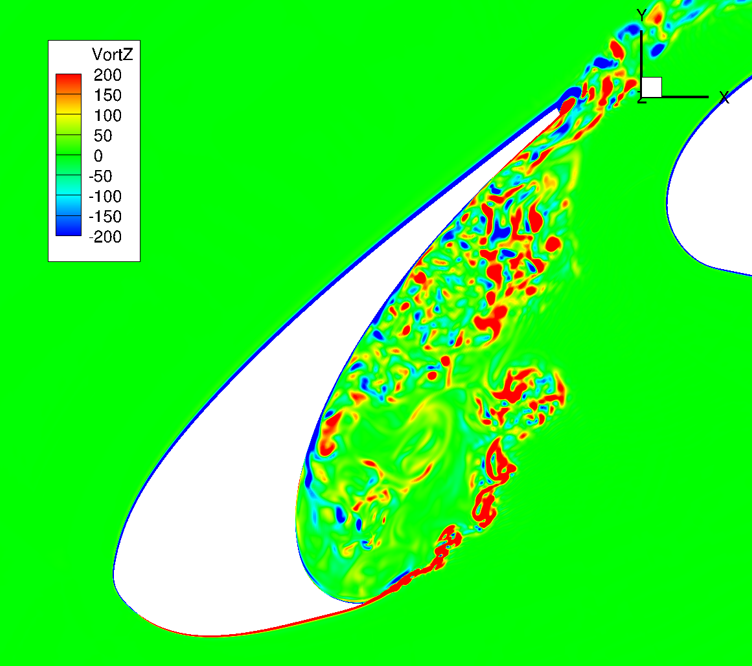
\includegraphics[width=\textwidth,height=2.65cm,keepaspectratio]
        {FIGURES/CHAMPS_APPLICATIONS/DDES.png}

        \vspace{0.05cm}
        \textbf{Scale-Resolving CFD (DDES)}
    \end{column}
    \hfill

    % Contrails
    \begin{column}{0.19\textwidth}
        \centering
        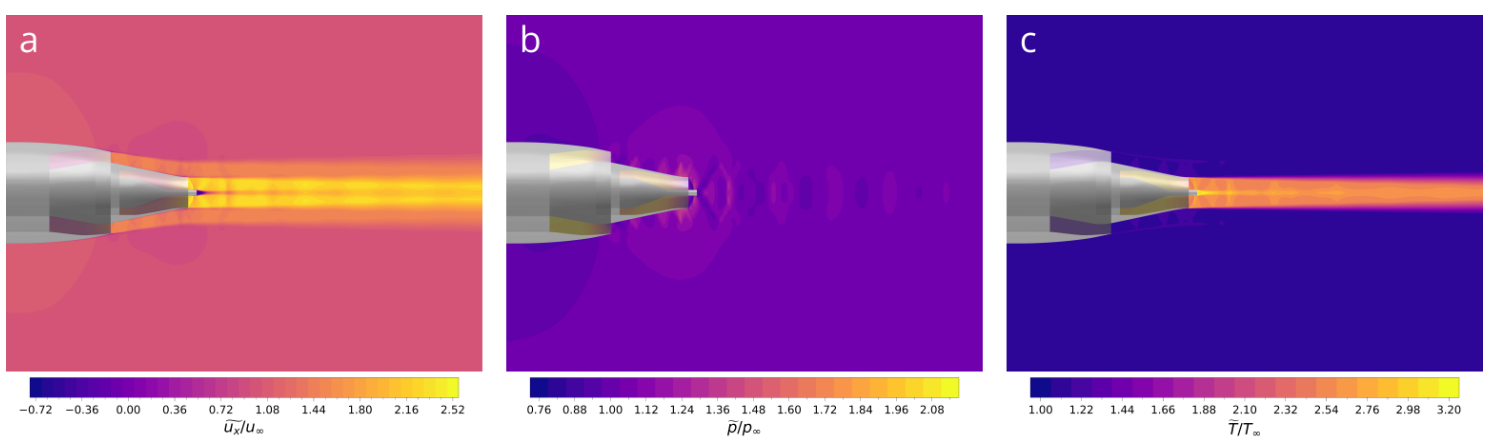
\includegraphics[width=\textwidth,height=2.65cm,keepaspectratio]
        {FIGURES/CHAMPS_APPLICATIONS/CONTRAILS.png}

        \vspace{0.05cm}
        \textbf{Contrails}$^{*}$
    \end{column}
    \hfill

    % Stochastic icing
    \begin{column}{0.19\textwidth}
        \centering
        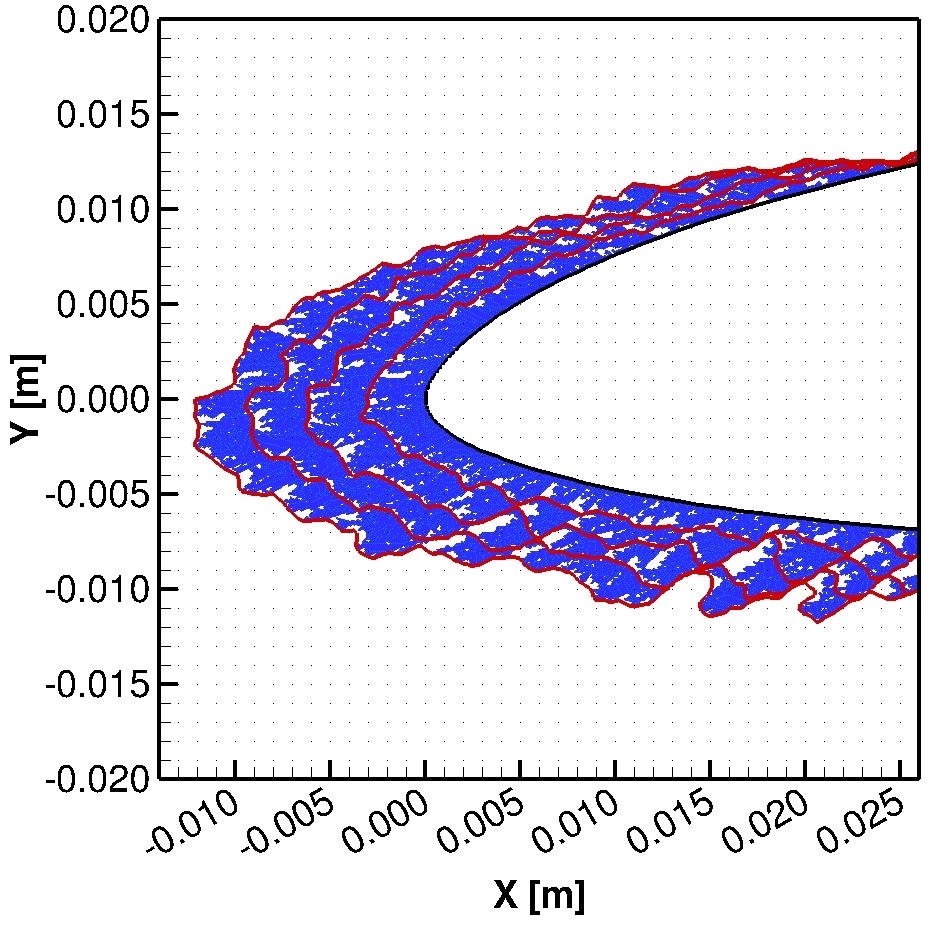
\includegraphics[width=\textwidth,height=2.65cm,keepaspectratio]
        {FIGURES/CHAMPS_APPLICATIONS/STOCHASTIC_ICING.jpeg}

        \vspace{0.05cm}
        \textbf{Stochastic Icing}
    \end{column}
    \hfill

    % FSI placeholder
    \begin{column}{0.19\textwidth}
        \centering

        \fbox{%
            \parbox[c][2.55cm][c]{0.94\textwidth}{%
                \centering
                \Large FSI\\[0.15cm]
                \scriptsize Figure Placeholder
            }%
        }

        \vspace{0.05cm}
        \textbf{Fluid--Structure Interaction}
    \end{column}

\end{columns}

\vspace{0.15cm}

{\tiny
$^{*}$Contrail modeling developed in collaboration with Prof.\ Roberto Paoli.
}

\end{frame}

% ============================================================
% CHAMPS -- Overview
% ============================================================

\begin{frame}{\textbf{CHAMPS: Advanced 2D-3D CFD Solver}}
\scriptsize
\begin{block}{ \small \textbf{CHAMPS (CHapel MultiPhysics Software)}}
\begin{itemize}
\item 2D-3D Unstructured Reynolds Average Navier Stokes Solver
\item Second order finite volume 
\item Convective Fluxes : Roe, AUSM
\item SA, k-$\omega$ SST-V and Langtry-Menter transitional turbulence models
\item Explicit solver (Runge-Kutta) and implicit solvers (SGS, GMRES)
\item Linked to external libraries: MKL, CGNS, METIS and PETSC
\item Multi-Fidelity Solvers: Potential, Non Linear Vortex Lattice, Euler, RANS, URANS, LES, DNS
\item Multi-Physics: Icing (Deterministic, Stochastic), Fluid-Structure Interactions, Contrails
\end{itemize}
\end{block}

\begin{alertblock}{ \small \textbf{CHAMPS Software : 150,000 lines of code !}}
\begin{itemize}
    \item Pre-Processor $\approx$ 17K lines
    \item Post Processor $\approx$ 2K lines
    \item Flow Solver $\approx$ 15K lines
    \item Turbulence Solver $\approx$ 13K lines
    \item Droplet Solver (Eulerian + Lagrangian) $\approx$ 24K lines
    \item Fluid-Structure Interaction Solver (Coupling + FEM) $\approx$ 15K lines
    
    
\end{itemize}
\end{alertblock}
\end{frame}